\chapter{Branching e Merging}

\section*{Introduzione}
Il branching è una delle feature killer di Git. Permette di divergere dalla linea principale di sviluppo per lavorare su feature, esperimenti o fix senza impattare il codice stabile. Questo capitolo copre creazione branch, switching, merging, rebase e risoluzione conflitti.

\section*{Obiettivi di apprendimento}
\begin{itemize}
    \item Comprendere cosa sono i branch e perché sono fondamentali
    \item Creare e gestire branch (\texttt{git branch})
    \item Switching tra branch (\texttt{git checkout}/\texttt{git switch})
    \item Merge: fast-forward e three-way merge
    \item Rebase per linearizzare la storia
    \item Risolvere conflitti di merge
    \item Eliminare branch obsoleti
    \item Best practices per branching strategy
\end{itemize}

\section{Cosa Sono i Branch}

\subsection{Definizione}

Un \textbf{branch} (ramo) in Git è semplicemente un puntatore mobile a un commit. Il branch di default è chiamato \texttt{main} (o \texttt{master} in repo più vecchi).

\begin{figure}[h]
    \centering
    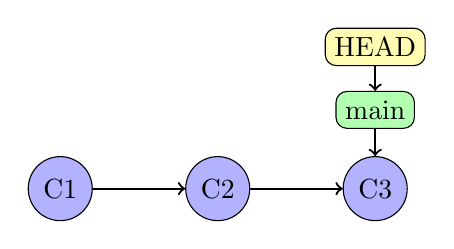
\begin{tikzpicture}[
        commit/.style={circle, draw, fill=blue!30, minimum size=0.8cm},
        branch/.style={rectangle, draw, fill=green!30, rounded corners},
        arrow/.style={->, thick}
    ]
        % Commits
        \node[commit] (c1) at (0,0) {C1};
        \node[commit] (c2) at (2,0) {C2};
        \node[commit] (c3) at (4,0) {C3};

        % Branch pointer
        \node[branch] (main) at (4,1) {main};

        % HEAD pointer
        \node[branch, fill=yellow!30] (head) at (4,1.8) {HEAD};

        % Arrows
        \draw[arrow] (c1) -- (c2);
        \draw[arrow] (c2) -- (c3);
        \draw[arrow] (main) -- (c3);
        \draw[arrow] (head) -- (main);
    \end{tikzpicture}
    \caption{Branch come puntatore a commit}
\end{figure}

\textbf{Concetti chiave}:
\begin{itemize}
    \item \textbf{Branch}: Puntatore a un commit specifico
    \item \textbf{HEAD}: Puntatore al branch corrente (dove sei ora)
    \item Creare branch è \textbf{istantaneo} (solo creare puntatore)
    \item Nessun overhead di copia file
\end{itemize}

\subsection{Perché usare i branch}

\begin{tcolorbox}[colback=green!10, colframe=green!60, title=Vantaggi del Branching]
\begin{itemize}
    \item \textbf{Isolamento}: Lavora su feature senza toccare codice stabile
    \item \textbf{Sperimentazione}: Prova idee senza rischio
    \item \textbf{Collaborazione}: Team lavora su feature diverse in parallelo
    \item \textbf{Code review}: Feature branch + pull request
    \item \textbf{Hotfix}: Fixa bug in produzione senza feature incomplete
    \item \textbf{Release management}: Branch per versioni diverse
\end{itemize}
\end{tcolorbox}

\begin{tcolorbox}[colback=blue!10, colframe=blue!60, title=Scenario Tipico]
Stai sviluppando feature complessa (richiederà 2 settimane). Nel frattempo:
\begin{enumerate}
    \item Bug critico scoperto in produzione
    \item Altro dev aggiunge piccola feature
    \item Testing richiede modifiche
\end{enumerate}

Senza branch: chaos totale, conflitti continui, impossibile deployare.

Con branch:
\begin{itemize}
    \item \texttt{main}: codice stabile in produzione
    \item \texttt{feature/nuova-ui}: tua feature (isolata)
    \item \texttt{hotfix/critical-bug}: fix urgente
    \item \texttt{feature/small-feature}: altra feature
\end{itemize}

Ogni branch evolve indipendentemente, merge quando pronto!
\end{tcolorbox}

\section{Creare e Gestire Branch}

\subsection{Visualizzare branch esistenti}

\begin{lstlisting}[caption=Listare branch]
# Lista branch locali
$ git branch
* main
  feature/login
  hotfix/navbar

# Branch con ultimo commit
$ git branch -v
* main           a3f5b21 Add user authentication
  feature/login  b8c9d34 WIP: login form
  hotfix/navbar  c7e2a19 Fix navbar on mobile

# Lista branch locali e remoti
$ git branch -a
* main
  feature/login
  remotes/origin/main
  remotes/origin/develop

# Branch merged/non-merged
$ git branch --merged        # Branch già mergiati in corrente
$ git branch --no-merged     # Branch non ancora mergiati
\end{lstlisting}

\subsection{Creare branch}

\begin{lstlisting}[caption=Creare nuovo branch]
# Crea branch (non switcha)
$ git branch feature/nuova-feature

# Verifica creazione
$ git branch
* main
  feature/nuova-feature

# Crea e switcha in un comando (metodo classico)
$ git checkout -b feature/altra-feature
Switched to a new branch 'feature/altra-feature'

# Crea e switcha (Git 2.23+, raccomandato)
$ git switch -c feature/moderna-feature
Switched to a new branch 'feature/moderna-feature'

# Crea branch da commit specifico
$ git branch hotfix/bug a3f5b21

# Crea branch da tag
$ git branch release/v2.0 v2.0
\end{lstlisting}

\subsection{Switching tra branch}

\begin{lstlisting}[caption=Cambiare branch]
# Metodo classico
$ git checkout feature/nuova-feature
Switched to branch 'feature/nuova-feature'

# Metodo moderno (Git 2.23+)
$ git switch feature/nuova-feature
Switched to branch 'feature/nuova-feature'

# Torna al branch precedente
$ git switch -

# Switcha e crea se non esiste
$ git switch -c feature/auto-create
\end{lstlisting}

\begin{tcolorbox}[colback=orange!10, colframe=orange!60, title=Nota: checkout vs switch]
Git 2.23 (2019) ha introdotto \texttt{git switch} per rendere più chiara la separazione:
\begin{itemize}
    \item \texttt{git switch}: Cambiare branch
    \item \texttt{git restore}: Ripristinare file
    \item \texttt{git checkout}: Fa entrambi (confusionario)
\end{itemize}

Raccomandazione: usa \texttt{switch} e \texttt{restore} nei nuovi progetti.
\end{tcolorbox}

\subsection{Rinominare branch}

\begin{lstlisting}[caption=Rinominare branch]
# Rinomina branch corrente
$ git branch -m nuovo-nome

# Rinomina branch specifico
$ git branch -m vecchio-nome nuovo-nome

# Esempio: rinomina master in main
$ git branch -m master main
\end{lstlisting}

\subsection{Eliminare branch}

\begin{lstlisting}[caption=Eliminare branch]
# Elimina branch (safe: solo se merged)
$ git branch -d feature/completata
Deleted branch feature/completata (was a3f5b21).

# Force delete (anche se non merged)
$ git branch -D feature/abbandonata
Deleted branch feature/abbandonata (was b8c9d34).

# Elimina branch remoto
$ git push origin --delete feature/vecchia
\end{lstlisting}

\begin{tcolorbox}[colback=red!10, colframe=red!60, title=Attenzione: Branch Deletion]
\texttt{-d} è safe: Git impedisce eliminazione se branch non merged (protezione da perdita lavoro). \texttt{-D} è force: elimina anche branch non merged. Usa \texttt{-D} solo se sei sicuro di voler perdere quel lavoro.
\end{tcolorbox}

\section{Merging: Unire Branch}

\subsection{Concetto di merge}

\textbf{Merge} integra modifiche da un branch in un altro. Tipicamente: merge feature branch in \texttt{main}.

\subsection{Fast-Forward Merge}

Quando non ci sono commit divergenti, Git fa \textbf{fast-forward}: sposta semplicemente puntatore avanti.

\begin{figure}[h]
    \centering
    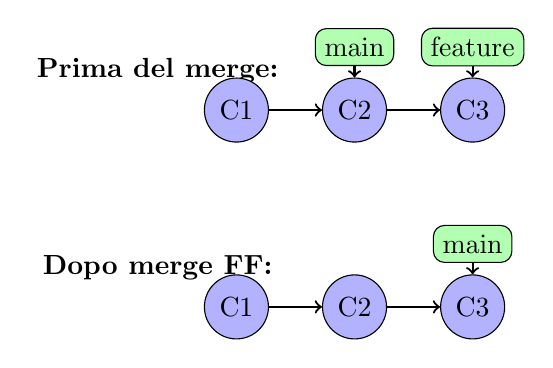
\begin{tikzpicture}[
        commit/.style={circle, draw, fill=blue!30, minimum size=0.8cm},
        branch/.style={rectangle, draw, fill=green!30, rounded corners},
        arrow/.style={->, thick}
    ]
        % Before merge
        \node at (-1, 2.5) {\textbf{Prima del merge:}};
        \node[commit] (c1) at (0,2) {C1};
        \node[commit] (c2) at (1.5,2) {C2};
        \node[commit] (c3) at (3,2) {C3};

        \node[branch] (main) at (1.5,2.8) {main};
        \node[branch] (feature) at (3,2.8) {feature};

        \draw[arrow] (c1) -- (c2);
        \draw[arrow] (c2) -- (c3);
        \draw[arrow] (main) -- (c2);
        \draw[arrow] (feature) -- (c3);

        % After merge
        \node at (-1, 0) {\textbf{Dopo merge FF:}};
        \node[commit] (c1b) at (0,-0.5) {C1};
        \node[commit] (c2b) at (1.5,-0.5) {C2};
        \node[commit] (c3b) at (3,-0.5) {C3};

        \node[branch] (mainb) at (3,0.3) {main};

        \draw[arrow] (c1b) -- (c2b);
        \draw[arrow] (c2b) -- (c3b);
        \draw[arrow] (mainb) -- (c3b);
    \end{tikzpicture}
    \caption{Fast-Forward Merge}
\end{figure}

\begin{lstlisting}[caption=Esempio Fast-Forward Merge]
# Situazione iniziale
$ git log --oneline --graph --all
* c3 (feature) Add feature C
* c2 Add feature B
* c1 (HEAD -> main) Initial commit

# Merge feature in main
$ git switch main
$ git merge feature
Updating c1..c3
Fast-forward
 feature.py | 10 ++++++++++
 1 file changed, 10 insertions(+)

# Storia dopo merge
$ git log --oneline --graph
* c3 (HEAD -> main, feature) Add feature C
* c2 Add feature B
* c1 Initial commit
\end{lstlisting}

\textbf{Caratteristiche FF merge}:
\begin{itemize}
    \item Nessun commit di merge creato
    \item Storia lineare e pulita
    \item Possibile solo se nessun commit divergente
\end{itemize}

\subsection{Three-Way Merge}

Quando i branch hanno commit divergenti, Git crea \textbf{merge commit} con due parent.

\begin{figure}[h]
    \centering
    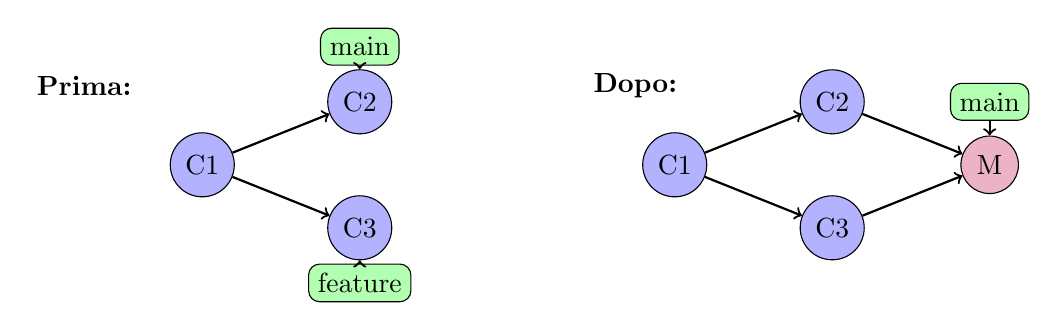
\begin{tikzpicture}[
        commit/.style={circle, draw, fill=blue!30, minimum size=0.7cm},
        branch/.style={rectangle, draw, fill=green!30, rounded corners},
        arrow/.style={->, thick}
    ]
        % Before merge
        \node at (-1.5, 3) {\textbf{Prima:}};
        \node[commit] (c1) at (0,2) {C1};
        \node[commit] (c2) at (2,2.8) {C2};
        \node[commit] (c3) at (2,1.2) {C3};

        \node[branch] (main) at (2,3.5) {main};
        \node[branch] (feat) at (2,0.5) {feature};

        \draw[arrow] (c1) -- (c2);
        \draw[arrow] (c1) -- (c3);
        \draw[arrow] (main) -- (c2);
        \draw[arrow] (feat) -- (c3);

        % After merge
        \node at (5.5, 3) {\textbf{Dopo:}};
        \node[commit] (c1b) at (6,2) {C1};
        \node[commit] (c2b) at (8,2.8) {C2};
        \node[commit] (c3b) at (8,1.2) {C3};
        \node[commit, fill=purple!30] (c4) at (10,2) {M};

        \node[branch] (mainb) at (10,2.8) {main};

        \draw[arrow] (c1b) -- (c2b);
        \draw[arrow] (c1b) -- (c3b);
        \draw[arrow] (c2b) -- (c4);
        \draw[arrow] (c3b) -- (c4);
        \draw[arrow] (mainb) -- (c4);
    \end{tikzpicture}
    \caption{Three-Way Merge (M = merge commit)}
\end{figure}

\begin{lstlisting}[caption=Esempio Three-Way Merge]
# Situazione: main e feature divergenti
$ git log --oneline --graph --all
* c3 (feature) Add feature C
| * c2 (HEAD -> main) Fix bug in main
|/
* c1 Initial commit

# Merge feature in main
$ git switch main
$ git merge feature
Merge made by the 'recursive' strategy.
 feature.py | 10 ++++++++++
 1 file changed, 10 insertions(+)

# Storia dopo merge
$ git log --oneline --graph
*   m1 (HEAD -> main) Merge branch 'feature'
|\
| * c3 (feature) Add feature C
* | c2 Fix bug in main
|/
* c1 Initial commit
\end{lstlisting}

\textbf{Caratteristiche three-way merge}:
\begin{itemize}
    \item Crea merge commit con due parent
    \item Messaggio auto-generato (modificabile)
    \item Preserva storia non lineare
    \item Mostra chiaramente quando feature fu integrata
\end{itemize}

\subsection{Forzare merge commit (no fast-forward)}

\begin{lstlisting}[caption=Merge con --no-ff]
# Forza creazione merge commit anche se FF possibile
$ git merge --no-ff feature/login

# Utile per preservare informazione "questa era una feature"
$ git log --oneline --graph
*   m1 (HEAD -> main) Merge branch 'feature/login'
|\
| * c3 (feature/login) Complete login form
| * c2 Add login validation
|/
* c1 Initial commit
\end{lstlisting}

\begin{tcolorbox}[colback=green!10, colframe=green!60, title=Best Practice: --no-ff per Feature]
In workflow professionali (Git Flow), è comune usare \texttt{--no-ff} per feature branch. Mantiene traccia chiara di quando feature fu aggiunta. Storia mostra:
\begin{itemize}
    \item Quali commit fanno parte della feature
    \item Quando fu integrata
    \item Facile revert intera feature (revert del merge commit)
\end{itemize}
\end{tcolorbox}

\subsection{Merge squash}

\begin{lstlisting}[caption=Merge con squash]
# Merge tutti commit feature in singolo commit
$ git merge --squash feature/experiment
Squash commit -- not updating HEAD
Automatic merge went well; stopped before committing as requested

$ git commit -m "Add experimental feature"

# Storia risultante: un solo commit, non merge commit
$ git log --oneline
* m1 (HEAD -> main) Add experimental feature
* c1 Initial commit
\end{lstlisting}

\textbf{Quando usare squash}:
\begin{itemize}
    \item Feature con molti commit WIP disordinati
    \item Vuoi storia main pulita e lineare
    \item Commit intermedi non aggiungono valore
\end{itemize}

\textbf{Svantaggio}: Perdi storia dettagliata feature development.

\section{Conflitti di Merge}

\subsection{Quando avvengono conflitti}

Conflitto avviene quando:
\begin{itemize}
    \item Due branch modificano stessa riga di stesso file
    \item Un branch modifica file, altro lo elimina
    \item Rename complessi
\end{itemize}

\subsection{Esempio conflitto}

\begin{lstlisting}[caption=Merge con conflitto]
$ git merge feature/conflict
Auto-merging main.py
CONFLICT (content): Merge conflict in main.py
Automatic merge failed; fix conflicts and then commit the result.

$ git status
On branch main
You have unmerged paths.
  (fix conflicts and run "git commit")

Unmerged paths:
  (use "git add <file>..." to mark resolution)
        both modified:   main.py
\end{lstlisting}

\subsection{Formato marker conflitto}

\begin{lstlisting}[caption=File con conflitto]
def greet():
<<<<<<< HEAD
    print("Hello from main!")
=======
    print("Hello from feature!")
>>>>>>> feature/conflict
    return True
\end{lstlisting}

\textbf{Marker conflitto}:
\begin{itemize}
    \item \texttt{<<<<<<< HEAD}: Inizio versione branch corrente
    \item \texttt{=======}: Separatore
    \item \texttt{>>>>>>> feature}: Fine versione branch da mergere
\end{itemize}

\subsection{Risolvere conflitti}

\textbf{Processo risoluzione}:

\begin{enumerate}
    \item \textbf{Identifica file}: \texttt{git status} mostra "both modified"
    \item \textbf{Apri file}: Cerca marker \texttt{<<<<<<<}
    \item \textbf{Decidi versione}: Mantieni una, entrambe, o scrivi nuova
    \item \textbf{Rimuovi marker}: Elimina \texttt{<<<<<<<}, \texttt{=======}, \texttt{>>>>>>>}
    \item \textbf{Stage file}: \texttt{git add main.py}
    \item \textbf{Completa merge}: \texttt{git commit}
\end{enumerate}

\begin{lstlisting}[caption=Risoluzione conflitto manuale]
# 1. Vedi conflitti
$ git status
Unmerged paths:
        both modified:   main.py

# 2. Modifica file (scegli versione)
# Versione risolta:
def greet():
    print("Hello from both branches!")
    return True

# 3. Stage file risolto
$ git add main.py

# 4. Verifica risoluzione completa
$ git status
All conflicts fixed but you are still merging.
  (use "git commit" to conclude merge)

# 5. Completa merge
$ git commit
# Editor apre con messaggio auto-generato
[main a4b6c8d] Merge branch 'feature/conflict'
\end{lstlisting}

\subsection{Tool per risoluzione conflitti}

\begin{lstlisting}[caption=Usare merge tool]
# Configura merge tool (es: vimdiff, meld, kdiff3)
$ git config --global merge.tool vimdiff

# Lancia merge tool su conflitti
$ git mergetool

# Tool mostra 3 panel:
# - LOCAL (tua versione)
# - REMOTE (versione da mergere)
# - BASE (ancestor comune)
# - MERGED (risultato)
\end{lstlisting}

\subsection{Abortire merge}

\begin{lstlisting}[caption=Annullare merge in corso]
# Se merge non riesce e vuoi annullare tutto
$ git merge --abort

# Torna allo stato pre-merge
$ git status
On branch main
nothing to commit, working tree clean
\end{lstlisting}

\section{Rebase: Storia Lineare}

\subsection{Cos'è rebase}

\textbf{Rebase} riscrive la storia spostando commit su nuova base. Alternativa a merge per integrare modifiche.

\begin{figure}[h]
    \centering
    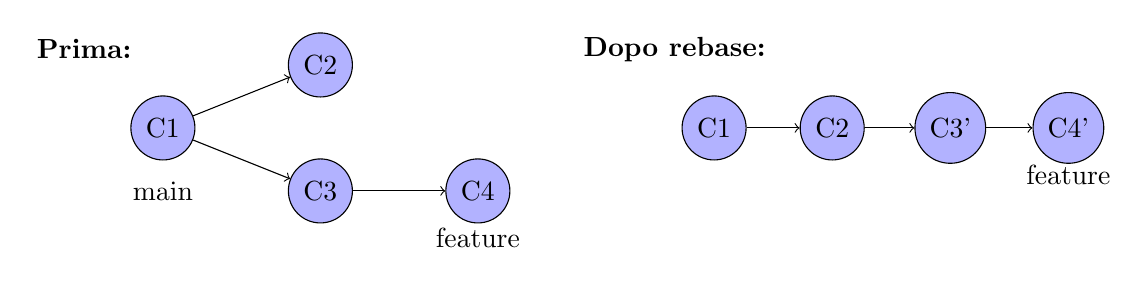
\begin{tikzpicture}[
        commit/.style={circle, draw, fill=blue!30, minimum size=0.7cm},
        arrow/.style={->, thick}
    ]
        % Before rebase
        \node at (-1, 3) {\textbf{Prima:}};
        \node[commit] (c1) at (0,2) {C1};
        \node[commit] (c2) at (2,2.8) {C2};
        \node[commit] (c3) at (2,1.2) {C3};
        \node[commit] (c4) at (4,1.2) {C4};

        \draw[->] (c1) -- (c2);
        \draw[->] (c1) -- (c3);
        \draw[->] (c3) -- (c4);

        \node at (0,1.2) {main};
        \node at (4,0.6) {feature};

        % After rebase
        \node at (6.5, 3) {\textbf{Dopo rebase:}};
        \node[commit] (c1b) at (7,2) {C1};
        \node[commit] (c2b) at (8.5,2) {C2};
        \node[commit] (c3b) at (10,2) {C3'};
        \node[commit] (c4b) at (11.5,2) {C4'};

        \draw[->] (c1b) -- (c2b);
        \draw[->] (c2b) -- (c3b);
        \draw[->] (c3b) -- (c4b);

        \node at (11.5,1.4) {feature};
    \end{tikzpicture}
    \caption{Rebase: C3' e C4' sono nuovi commit (hash diversi)}
\end{figure}

\subsection{Rebase base}

\begin{lstlisting}[caption=Rebase feature su main]
# Situazione iniziale
$ git log --oneline --graph --all
* c4 (feature) Add feature part 2
* c3 Add feature part 1
| * c2 (main) Fix bug
|/
* c1 Initial commit

# Switch a feature e rebase su main
$ git switch feature
$ git rebase main
First, rewinding head to replay your work on top of it...
Applying: Add feature part 1
Applying: Add feature part 2

# Storia dopo rebase (lineare!)
$ git log --oneline --graph
* c4' (HEAD -> feature) Add feature part 2
* c3' Add feature part 1
* c2 (main) Fix bug
* c1 Initial commit
\end{lstlisting}

\subsection{Rebase vs Merge}

\begin{tcolorbox}[colback=purple!10, colframe=purple!60, title=Merge vs Rebase]
\textbf{Merge}:
\begin{itemize}
    \item[+] Preserva storia vera del progetto
    \item[+] Safe: non riscrive commit esistenti
    \item[+] Mostra quando branch fu integrato
    \item[-] Storia non lineare (più complessa)
    \item[-] Molti merge commit possono inquinare storia
\end{itemize}

\textbf{Rebase}:
\begin{itemize}
    \item[+] Storia lineare e pulita
    \item[+] Facile da leggere e navigare
    \item[+] Nessun merge commit extra
    \item[-] Riscrive storia (cambia hash commit)
    \item[-] Può causare problemi su branch condivisi
\end{itemize}
\end{tcolorbox}

\subsection{Golden Rule of Rebase}

\begin{tcolorbox}[colback=red!10, colframe=red!60, title=REGOLA D'ORO: Mai Rebase Branch Pubblici]
\textbf{Mai fare rebase di commit già pushati su branch condivisi!}

Rebase riscrive storia (cambia hash). Se altri hanno già pullato quei commit, creerai caos:
\begin{itemize}
    \item Altri avranno commit duplicati
    \item Merge conflicts continui
    \item Storia corrotta e confusa
\end{itemize}

\textbf{Safe}: Rebase solo branch locali privati prima di pushare.

\textbf{Unsafe}: Rebase di \texttt{main} o branch condivisi.
\end{tcolorbox}

\subsection{Rebase interattivo}

\begin{lstlisting}[caption=Rebase interattivo per pulire storia]
# Rebase interattivo ultimi 3 commit
$ git rebase -i HEAD~3

# Editor apre con lista commit:
pick c3 Add feature part 1
pick c4 Fix typo
pick c5 Add feature part 2

# Comandi disponibili:
# pick = usa commit
# reword = usa commit ma modifica messaggio
# edit = usa commit ma fermati per amend
# squash = unisci con commit precedente
# fixup = come squash ma scarta messaggio
# drop = elimina commit

# Esempio: squash fix typo in commit precedente
pick c3 Add feature part 1
fixup c4 Fix typo
pick c5 Add feature part 2

# Salva e chiudi: Git applica modifiche
\end{lstlisting}

\textbf{Use case rebase interattivo}:
\begin{itemize}
    \item Pulizia storia prima di PR (squash WIP commits)
    \item Riordinare commit logicamente
    \item Correggere messaggi commit
    \item Eliminare commit di debug
\end{itemize}

\subsection{Rebase con conflitti}

\begin{lstlisting}[caption=Risolvere conflitti durante rebase]
$ git rebase main
Applying: Add feature
CONFLICT (content): Merge conflict in main.py

# Risolvi conflitti manualmente
$ vim main.py  # Risolvi e rimuovi marker

# Stage file risolto
$ git add main.py

# Continua rebase
$ git rebase --continue

# Oppure abbandona rebase
$ git rebase --abort
\end{lstlisting}

\section*{Riepilogo concetti chiave}

\begin{tcolorbox}[colback=gray!10, colframe=black!60, title=Concetti fondamentali]
\begin{itemize}
    \item \textbf{Branch} è un puntatore mobile a commit
    \item \texttt{git branch} crea/lista branch, \texttt{git switch} cambia branch
    \item \textbf{Merge} integra modifiche da branch: FF o three-way
    \item \textbf{Conflitti} avvengono quando stessa riga modificata in entrambi
    \item Risolvi conflitti manualmente, poi \texttt{git add} e \texttt{git commit}
    \item \textbf{Rebase} riscrive storia per renderla lineare
    \item \texttt{--no-ff} forza merge commit (utile per feature)
    \item \texttt{--squash} comprime branch in singolo commit
    \item \textbf{Golden Rule}: Mai rebase branch pubblici condivisi
    \item Rebase interattivo (\texttt{-i}) per pulizia storia
\end{itemize}
\end{tcolorbox}

\section*{Esercizi}

\begin{enumerate}
    \item Crea branch \texttt{feature/test}, aggiungi 2 commit, mergia in \texttt{main}.

    \item Crea due branch divergenti, fai three-way merge, visualizza con \texttt{git log --graph}.

    \item Crea conflitto intenzionale (modifica stessa riga in due branch), risolvi manualmente.

    \item Usa \texttt{git merge --no-ff} e confronta storia con merge FF.

    \item Crea branch con 5 commit, usa rebase interattivo per squashare in 2 commit.

    \item Sperimenta \texttt{git rebase} per linearizzare storia.

    \item Simula scenario: branch \texttt{main} avanza, feature branch diventa outdated, rebase feature su main.

    \item Usa \texttt{git mergetool} (configura prima tool preferito).

    \item Crea alias per \texttt{git log --graph --oneline --all}.

    \item Pratica workflow: crea feature branch, sviluppa, rebase su main aggiornato, merge.
\end{enumerate}

\section*{Riferimenti}

\begin{itemize}
    \item Git Branching: \url{https://git-scm.com/book/en/v2/Git-Branching-Branches-in-a-Nutshell}
    \item Merge vs Rebase: \url{https://www.atlassian.com/git/tutorials/merging-vs-rebasing}
    \item Resolving Conflicts: \url{https://git-scm.com/book/en/v2/Git-Branching-Basic-Branching-and-Merging}
\end{itemize}
